\section{Results}
\label{sec:results}

\subsection{Headline scaling table}

\Tabref{tab:headline} presents the central result of the paper. Across the \pythia family, standard categorical and relational knowledge consumes \(\mathbf{0.000061\%}\) (\(2.8\)B) to \(\mathbf{0.000224\%}\) (\(160\)M) of the model's bit budget at \(\beta = 2\) bpp --- between two and four parts per million of stored capacity. The conservative \(\beta = 3.6\) bpp denominator pushes the figure down by another \(\sim 45\%\) but does not change conclusions.

\begin{table}[t]
\centering
\caption{Standard-knowledge accuracy, acquired bits, and parameter share across the \pythia family. \bear and \taxi accuracies are macro-averages over the benchmark; bits are computed by \eqref{eq:bits}. \emph{Combined bits} sum \bear and \taxi acquired bits. Best (smallest) shares would correspond to most-diluted parameter footprints; we bold the headline figures at \(\beta = 2\) bpp.}
\label{tab:headline}
\resizebox{\textwidth}{!}{%
\begin{tabular}{@{}lrrrrrrrr@{}}
\toprule
\textbf{Model} & \textbf{Params} & \textbf{\bear acc} & \textbf{\taxi acc} & \textbf{\bear bits} & \textbf{\taxi bits} & \textbf{Combined bits} & \textbf{Share @ 2 bpp} & \textbf{Share @ 3.6 bpp} \\
\midrule
\pythiaA & 162M  & 6.14\%  & 23.48\% & 606.3   & 119.7  & 726   & \textbf{0.000224\%} & 0.000124\% \\
\pythiaB & 405M  & 8.87\%  & 28.08\% & 1543.5  & 218.5  & 1762  & \textbf{0.000217\%} & 0.000121\% \\
\pythiaC & 1.01B & 9.70\%  & 27.60\% & 1865.1  & 220.2  & 2085  & \textbf{0.000103\%} & 0.000057\% \\
\pythiaD & 2.78B & 13.05\% & 30.24\% & 3104.0  & 257.5  & 3361  & \textbf{0.000061\%} & 0.000034\% \\
\bottomrule
\end{tabular}%
}
\end{table}

Bootstrap \(95\%\) confidence intervals over per-fact resampling (\(400\) draws) confirm the trend is not a sampling artefact: \(0.000168\%\) (\([0.000109, 0.000223]\)) at \(160\)M, \(0.000197\%\) (\([0.000171, 0.000222]\)) at \(410\)M, \(0.000095\%\) (\([0.000083, 0.000106]\)) at \(1\)B, and \(0.000059\%\) (\([0.000053, 0.000064]\)) at \(2.8\)B. The intervals at \(1\)B and \(2.8\)B are \emph{disjoint} from those at \(160\)M and \(410\)M, so the parameter-share decay is statistically reliable despite only four model points. (The bootstrap point estimate sits below the analytical share because the analytical formula subtracts the per-relation random baseline inside the sum, while the bootstrap re-aggregates per-fact contributions.)

\subsection{Scaling regression}

\Tabref{tab:scaling} regresses acquired bits and parameter share on parameter count in log-log space. \bear bits scale with a slope of \(\mathbf{0.54}\) (\(R^2 = 0.92\), \(p = 0.04\)); combined bits with \(0.50\) (\(R^2 = 0.92\), \(p = 0.04\)). Both slopes are significantly less than \(1\): adding a parameter buys only \emph{half a fractional bit} of standard knowledge, far less than the one bit of capacity it adds at \(\beta = 2\) bpp. This is the mechanism by which the parameter share shrinks with scale --- standard-knowledge bits grow sub-linearly while capacity grows linearly. \taxi bits scale even more slowly (\(0.24\)), consistent with the saturation we discuss in \Secref{sec:results-surprises}.

\begin{table}[t]
\centering
\caption{Log-log scaling regressions. Slopes \(<1\) indicate sub-linear growth of acquired bits with parameter count, which forces the parameter share to shrink with scale. Source: \texttt{results/scaling\_regression.json}.}
\label{tab:scaling}
\begin{tabular}{@{}lrrr@{}}
\toprule
\textbf{Quantity} & \textbf{Slope} & \(R^2\) & \(p\) \\
\midrule
\bear bits acquired vs. params  & \textbf{0.54} & 0.92 & 0.039 \\
\taxi bits acquired vs. params  & 0.24 & 0.76 & 0.13 \\
Combined bits vs. params        & \textbf{0.50} & 0.92 & 0.042 \\
Share (\%) vs. \(\log_{10}\)(params) (linear)  & \(-0.000147\) pp/decade & 0.90 & 0.050 \\
\bottomrule
\end{tabular}
\end{table}

\subsection{Visualizations}

\Figref{fig:scaling_bits} plots acquired bits against parameter count in log-log space, with the \(2\) bpp and \(3.6\) bpp capacity ceilings drawn as reference lines. The probed-knowledge curve sits \(\mathbf{5}\)--\(\mathbf{6}\) orders of magnitude below the ceiling at every scale: even at \(2.8\)B, where we measure \(3.36 \times 10^3\) acquired bits, the model has \(5.56 \times 10^9\) bits of knowledge capacity available at \(\beta = 2\) bpp.

\begin{figure}[t]
\centering
\begin{subfigure}[b]{0.48\textwidth}
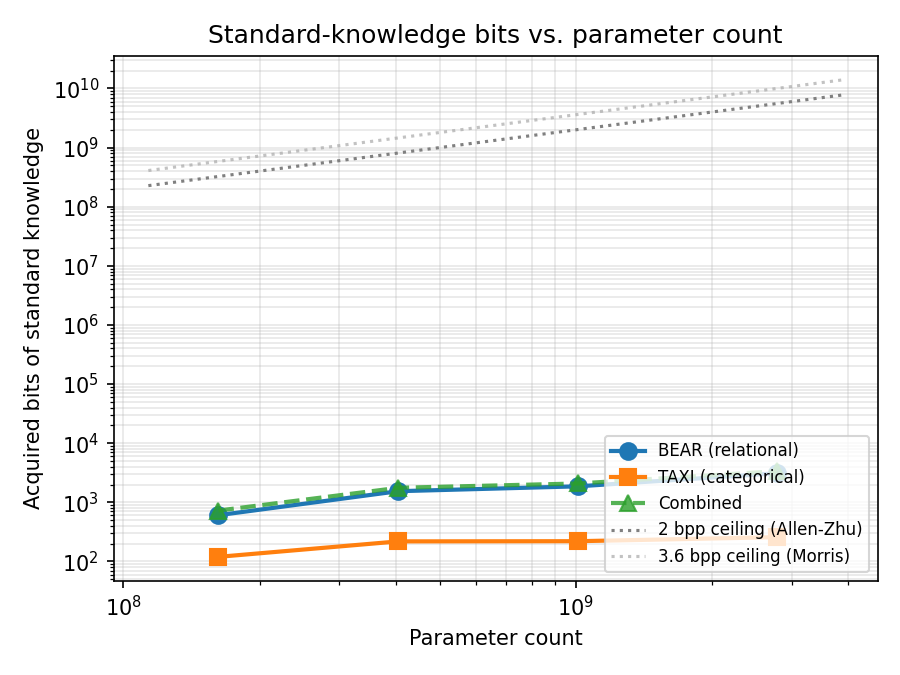
\includegraphics[width=\textwidth]{figures/scaling_bits.png}
\caption{Acquired bits vs. parameters. Standard-knowledge bits stay \(5\)--\(6\) orders of magnitude below the \(2\) bpp and \(3.6\) bpp capacity ceilings.}
\label{fig:scaling_bits}
\end{subfigure}\hfill
\begin{subfigure}[b]{0.48\textwidth}
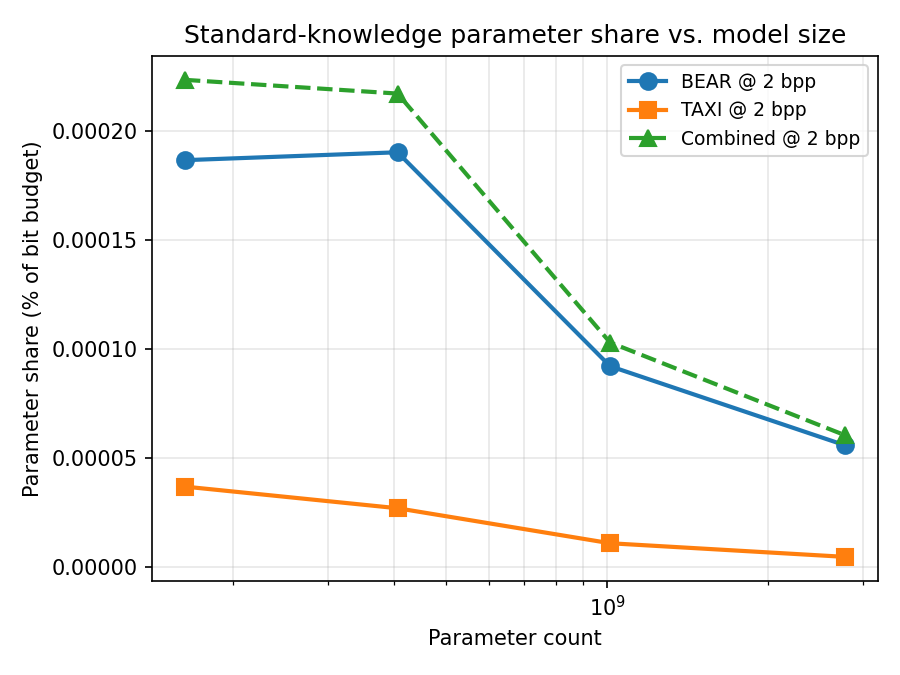
\includegraphics[width=\textwidth]{figures/scaling_share.png}
\caption{Parameter share (\% of bit budget). The combined share halves between \(410\)M and \(1\)B, and halves again from \(1\)B to \(2.8\)B.}
\label{fig:scaling_share}
\end{subfigure}
\caption{Scaling of standard-knowledge footprint across \pythia. \captiona acquired bits are far below capacity at every scale; \captionb the parameter share shrinks monotonically with model size from \(410\)M onward.}
\label{fig:scaling}
\end{figure}

\Figref{fig:bear_taxi} compares relational and categorical contributions: \bear contributes more aggregate bits than \taxi at every scale (purely because it has roughly five times more facts), but \taxi achieves higher per-fact accuracy. \Figref{fig:per_category} breaks \taxi down by superordinate category: \emph{animals} and \emph{foods} are the best-encoded categories across all model scales, with vehicles and instruments lagging behind.

\begin{figure}[t]
\centering
\begin{subfigure}[b]{0.48\textwidth}
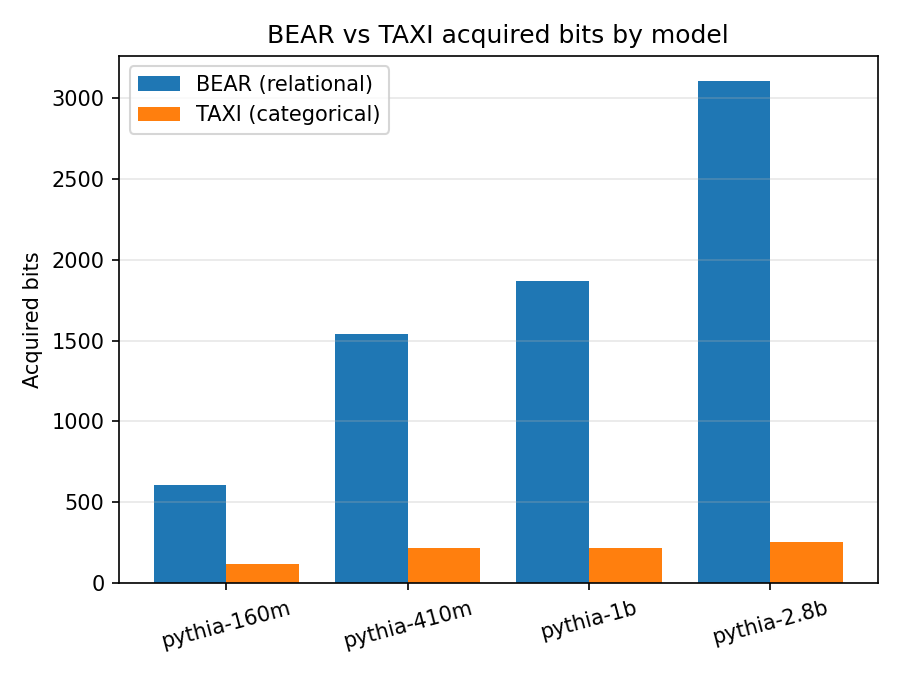
\includegraphics[width=\textwidth]{figures/bear_vs_taxi_bits.png}
\caption{\bear vs. \taxi acquired bits. \bear dominates the bit count by virtue of having roughly \(5\times\) more facts.}
\label{fig:bear_taxi}
\end{subfigure}\hfill
\begin{subfigure}[b]{0.48\textwidth}
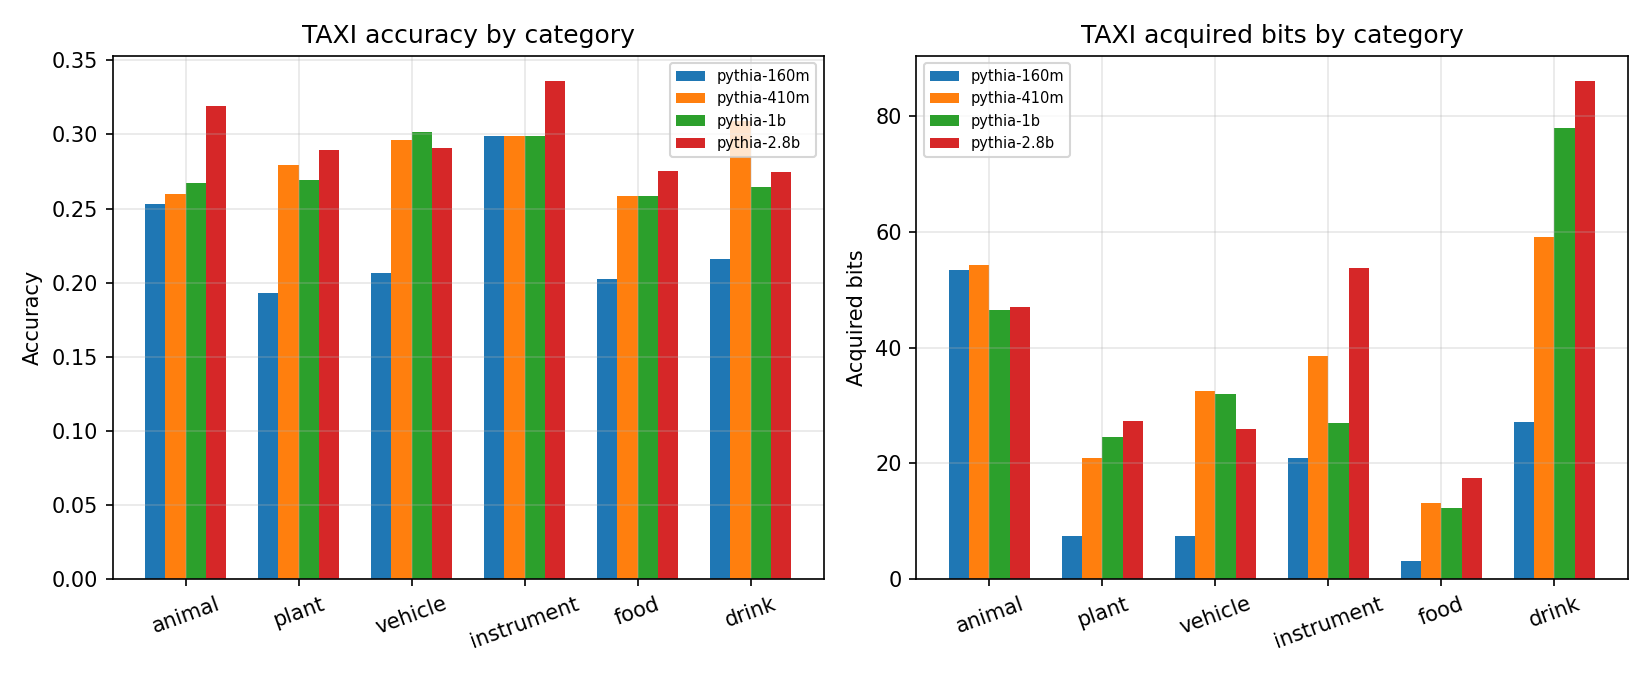
\includegraphics[width=\textwidth]{figures/per_category.png}
\caption{\taxi accuracy and acquired bits by superordinate category. \emph{Animals} and \emph{foods} are best-encoded across all scales.}
\label{fig:per_category}
\end{subfigure}
\caption{Knowledge-type and category breakdowns of acquired bits across \pythia.}
\label{fig:breakdowns}
\end{figure}

\subsection{Per-relation breakdown}

\Tabref{tab:bear_top} lists the five best-known relations at \pythiaB. The model knows ``classification level'' (\(28.7\%\)), ``head of government'' (\(26.7\%\)), and ``ownership'' (\(26.0\%\)) substantially better than the average \bear accuracy (\(8.9\%\)) --- exactly the high-frequency, textbook-standard relations one would expect to be over-represented in pretraining text. This is direct evidence that the benchmark is dominated by the kind of knowledge our hypothesis targets.

\begin{table}[t]
\centering
\caption{Top-5 best-known \bear relations on \pythiaB by accuracy. Source: \texttt{results/bear\_per\_relation.csv}.}
\label{tab:bear_top}
\begin{tabular}{@{}llrrr@{}}
\toprule
\textbf{Relation} & \textbf{Template} & \textbf{Answer set} & \textbf{Acc} & \textbf{Acquired bits} \\
\midrule
P105 & ``[X] is classified at the [Y] level.''   & 5  & 28.7\% & 30.2  \\
P6   & ``The head of government of [X] is [Y].'' & 60 & 26.7\% & 88.6  \\
P127 & ``[X] is owned by [Y].''                  & 25 & 26.0\% & 153.2 \\
P36  & ``The capital of [X] is [Y].''            & 60 & 20.0\% & 65.0  \\
P137 & ``[X] is operated by [Y].''               & 25 & 19.3\% & 106.8 \\
\bottomrule
\end{tabular}
\end{table}

\subsection{Per-fact-footprint cross-check}

\Tabref{tab:footprint} converts the per-fact bounds of \kn~\citep{dai2022knowledge} and \rome~\citep{meng2022rome} into aggregate parameter shares for the \emph{known} facts at each scale. These are upper bounds that assume exclusive parameter ownership per fact (no sharing). They sit between \(\mathbf{0.7\%}\) and \(\mathbf{3.1\%}\) --- four orders of magnitude above our bit-budget figure of \(\sim 10^{-4}\%\). The gap quantifies just how aggressively parameter sharing must be operating in modern LLMs: a single FFN value vector cannot ``own'' a single fact, otherwise the aggregate would exceed the bit-budget figure by the four-orders-of-magnitude shown here. This is consistent with the polysemantic-neuron picture of \citet{geva2021ffnkv} and the rising parameter specialization of \citet{hong2025specialization}.

\begin{table}[t]
\centering
\caption{Analytical per-fact-footprint upper bounds for the \emph{known} facts at each scale, vs. our bit-budget estimate. \kn assumes \(8\cdot d_{\text{model}}\) params/fact; \rome assumes \(d_{\text{model}}+d_{\text{inter}}\). Source: \texttt{results/per\_fact\_footprint.json}.}
\label{tab:footprint}
\begin{tabular}{@{}lrrrrr@{}}
\toprule
\textbf{Model} & \textbf{Known facts} & \textbf{Params/fact (KN)} & \textbf{KN share} & \textbf{ROME share} & \textbf{Bit-budget share} \\
\midrule
\pythiaA & 812   & 6{,}144  & 3.07\% & 1.92\% & \(\sim\)0.00022\% \\
\pythiaB & 1088  & 8{,}192  & 2.20\% & 1.37\% & \(\sim\)0.00022\% \\
\pythiaC & 1145  & 16{,}384 & 1.85\% & 1.16\% & \(\sim\)0.00010\% \\
\pythiaD & 1443  & 20{,}480 & 1.06\% & 0.67\% & \(\sim\)0.00006\% \\
\bottomrule
\end{tabular}
\end{table}

\subsection{Surprises}
\label{sec:results-surprises}

Three observations were not predicted by the literature review.

\para{\taxi accuracy plateaus near \(1\)B.} \pythiaB and \pythiaC have nearly identical \taxi accuracy (\(28.08\%\) vs.\ \(27.60\%\)) despite a \(2.5\times\) parameter increase. \pythiaD only improves to \(30.24\%\). Categorical knowledge appears to saturate at modest model sizes --- consistent with \citet{hong2025specialization}'s finding that specialization (rather than additional capacity) drives knowledge utilization in larger models.

\para{\bear accuracy keeps growing.} \(6.1\% \to 8.9\% \to 9.7\% \to 13.0\%\) across the four sizes. Relational knowledge, which is more entity-specific, benefits more from scale than categorical knowledge.

\para{Best-known relations are the most ``standard.''} P105 (taxonomic level), P6 (head of government), P36 (capital), P127 (ownership) are exactly the textbook examples --- direct confirmation that the benchmark is dominated by the kind of standard knowledge our hypothesis targets, and that the parameter-share figures are not artefacts of obscure-fact querying.
